\chapter{Evaluation} \label{sect:evaluation}

\section{MacroLab}

We evaluate MacroLab in four parts. First, we evaluate the
programming abstraction by showing that it is expressive enough to
implement canonical CPS applications, such as data
collection and object tracking. Second, we measure the overhead of
running MacroLab programs as compared with similar programs written
using nesC and TinyOS. Third, we deploy one MacroLab application in
multiple different scenarios and measure the effect of DSCD on
message cost. Finally, we evaluate the accuracy of the static cost
analyzer.

\subsection{Expressiveness of the Abstraction}\label{sect:expressiveness}

We evaluate the expressive power of our programming abstraction by
showing that it can be used concisely to implement two canonical
CPS applications: {\em tree-based data collection} in Surge~\cite{Gay}
and {\em object tracking} in the Pursuer-Evader Game
(PEG)~\cite{Sharp}. We selected these two applications because they
represent basic algorithms that have been incorporated into many other
CPS applications.  Table~\ref{table:LOC} presents a
comparison of the number of lines of code necessary to implement Surge
and PEG in MacroLab as compared to their original implementations in
nesC/TinyOS. The number of lines of code for the nesC/TinyOS
implementations of Surge and PEG were cited from previous
publications~\cite{Muller,Kothari}.  The MacroLab applications
are about one-fiftieth the size of equivalent nesC/TinyOS implementation
in terms of lines of code. This ratio is typical of the difference in
size between equivalent Matlab and C programs. MacroLab builds a
considerable amount of logic such as routing algorithms and vector
operations into the run-time system.  We thus claim that MacroLab
dramatically reduces the amount of code and therefore the amount of
development and maintenance time required to implement basic CPS
applications.

The MacroLab programming abstraction is suitable for many application
domains, but it cannot express algorithms that require explicit
message passing. For example, it cannot
easily be used to implement
routing protocols, time synchronization protocols, or other
distributed middleware libraries.  Instead, all of these operations must be
incorporated into the run-time system. Thus, MacroLab programs are 
limited to distributed operations that can be neatly stored in a
library and provided by some interface. We claim that this it not
a restricting requirement for most CPS software. However, it
can make it difficult to provide application-specific distributed
operations. Developers must encapsulate such functionality by extending 
the run-time system. Code movement 
in systems like Agilla~\cite{Fok} and EnviroSuite~\cite{Luo} might be
difficult to implement in MacroLab.

\begin{table}
\centering
\begin{minipage}{\columnwidth}
\centering
\begin{tabular}{|c|c|c|}
\cline{2-3}
\multicolumn{1}{c|}{}&MacroLab&nesC/TinyOS\\
\hline
Surge&7&400\\
\hline
PEG&19&780\\
\hline
\end{tabular}
\end{minipage}
\smallskip
\caption[Lines of code comparison]{Comparison of lines of code required for equivalent
functionality in two basic CPS applications.}
\label{table:LOC}
\end{table}

\subsubsection{Surge}\label{sect:surge}

Surge is a simple application that periodically collects sensor readings from
all nodes and routes them back to a base station.  The data collection aspect of
Surge has been widely utilized in many sensor network applications. In fact,
many applications, such as~\cite{Mainwaring,Juang,Selavo}, involve primarily
data collection and in many other applications, such as AlarmNet~\cite{Wood},
data collection plays an important role. Thus, it is essential that an
abstraction for sensor network programming make it easy to implement data
collection applications.  Figure~\ref{code:Surge} shows the source code for
Surge written in MacroLab.  In line~1, the run-time system is instantiated and
in lines~2 and~3, it is used to instantiate a vector of light sensors (one for
each node in the network) and a macrovector to hold the light values.  Line~4 is
the beginning of a loop that occurs every 1000 milliseconds.  The light sensors
are read in line 5 and the values are displayed at the base station in line 6.

There is hidden complexity in the interaction between lines 5 and 6. The
decomposer identifies that the sensor resources are on the nodes while
the {\tt BASE\_DISPLAY} function is only available on the base station.  It
therefore infers that the information created in line 5 must be routed
across machine boundaries in order to be used in line 6 and the
compiled version of the code automatically invokes the routing algorithm
via the {\tt remoteFeval} interface described in Section~\ref{sect:RTS}.
The high-level algorithm can be expressed in seven lines of MacroLab. 
The automatically generated microcode that runs on the nodes is closer
in size to the nesC/TinyOS implementation. 

\begin{figure}
  \begin{macrolab}
RTS = RunTimeSystem();
lSensors = SensorVector('lightSensor','uint16');
lightValues = Macrovector('uint16');
every(1000)
  lightValues =  sense(lSensors);
  BASE_DISPLAY(lightValues);
end
  \end{macrolab}
  \smallskip
  \hrule width 1\columnwidth
  \caption[MacroLab implementation of Surge]{A data collection application
    (Surge) in MacroLab.  {\tt BASE\_DISPLAY} is implemented within the RTS and
    sends a message to a base station for display.}
  \label{code:Surge}
\end{figure}

\subsubsection{Pursuer-Evader Game (PEG)}\label{sect:peg}

The Pursuer-Evader Game (PEG) is a distributed CPS application that detects and
reports the position of a moving object within a sensor field.  It is a
canonical application in the field of robotics research where multiple robots
(the pursuers) collectively determine the locations of one or more evaders and
attempt to corral them. This application has been adapted by the sensor network
community~\cite{Sharp,Brooks,Li} and represents the algorithmic capabilities
necessary for a number of canonical applications such as object tracking and
in-network filtering of false positives. It is widely used as an application for
the evaluation of sensor network programming abstractions and
architectures~\cite{Whitehousea,Kothari,Gnawali} since it is one of the largest
TinyOS applications and utilizes a number of relatively sophisticated concepts
for sensor networks.  Figure~\ref{code:PEG} shows an implementation of PEG in
MacroLab in which the network routes the location of the evader to a camera
which visually follows the evader. In line~1, the run-time system is
instantiated and in lines~2 and~3, it is used to instantiate a vector of
magnetometer sensors, one for each node in the network.  In line 5, a {\tt
  neighborReflection} macrovector is created that automatically reflects and
stores the values of each node's neighbors' {\tt magVal} elements if they are
within the threshold.  In the main loop, the sensors are sampled and each node's
neighbors' magnetometer readings are checked against a threshold value to see if
there are more than two neighboring nodes that sense the evader. If so, a leader
is chosen from amongst them by finding the node with the highest of all
magnetometer readings. Its ID is then passed to the {\tt CAMERAFOCUS} function,
which focuses the camera on the location of that node.  The purpose of this
example is to demonstrate that MacroLab can concisely represent efficient,
neighborhood-based, in-network processing. We do not elaborate on how to focus
the camera on the location of the leader node.


\begin{figure}  
  \begin{macrolab}
RTS = RunTimeSystem();
magSensors = SensorVector('MagSensor', 'uint16');
magVals = Macrovector('uint16');
THRESH = uint8(3);
nRefl = neighborReflection(magVals,magVals>THRESH)
every(1000)
  magVals =  sense(magSensors);
  nodes = find(nRefl > THRESH);
  rowSum = sum(~isnan(nRefl(nodes,:)),2)
  toCheck = find(rowSum>2);
  if(toCheck)
    maxID = find(magVals(nodes(toCheck)) ...
                 == max(nRefl(nodes,:),[],2));
  end
  leaderID = nodes(toCheck(maxID));
  if(leaderID)
    CAMERAFOCUS(leaderID);
  end
end
  \end{macrolab}
  \smallskip
  \hrule width 1\columnwidth
  \caption[MacroLab implementation of PEG]{A tracking application (PEG) in MacroLab. {\tt CAMERAFOCUS} is implemented
  within the RTS and sends a message to the camera, which is at the base station.}
  \label{code:PEG}
\end{figure}



\subsection{Performance Overhead} \label{sec:performance}

To evaluate the performance overhead of MacroLab, we measured the
resource consumption of the two applications described in
Section~\ref{sect:expressiveness} and compared it against existing
applications written in nesC/TinyOS.  We found that MacroLab programs
are very similar to TinyOS programs in terms of memory footprint,
execution speed, and power consumption.

The program size and heap size of two MacroLab programs is shown in
Table~\ref{table:CodeSize}, along with those of several existing TinyOS
programs.  The MacroLab programs actually have a smaller memory footprint than
their corresponding TinyOS implementations, both in terms of program memory and
RAM. While the TinyOS versions may be somewhat more feature rich, the MacroLab
versions are still not much larger than extremely simple TinyOS applications
such as {\tt SenseToRfm}.  Table \ref{table:CodeBreakdown} shows the breakdown
of our MacroLab programs' memory footprints.  This information was collected by
examining the symbol table of the final binary executables.  Therefore any
variables or code removed by compiler optimizations are not included. The vast
majority of the program size of MacroLab applications (approximately 17KB of ROM
and 600 bytes of RAM) is due to imported TinyOS libraries for multi-hop routing,
access to the Analog-to-Digital Converter (ADC), and the Timer.  The run-time
system module requires 558 bytes of program memory and 66 bytes of RAM.  For
both PEG and Surge, the application logic itelf required less than 1.3KB of ROM
and 150 bytes of RAM.


\begin{table}
  \centering
  \begin{minipage}{\columnwidth}
    \centering
    \begin{tabular}{|l|r|r|}
      \hline
      \multicolumn{1}{|c}{Application} & \multicolumn{1}{|c|}{Program Size} & \multicolumn{1}{c|}{Heap Size}\\
      \hline
      TelosB&49,152&10,240\\
      MICAz&131,072&4,096\\
      \hline
      Blink&2,472&38\\
      CountRadio&11,266&351\\
      Oscilloscope&9,034&335\\
      OscilloscopeRF&14,536&449\\
      SenseToRfm&14,248&403\\
      TOSBase&10,328&1,827\\
      \bf{MacroLab\_Surge}&19,374&669\\
      SurgeTelos&24,790&911\\
      \bf{MacroLab\_PEG}&18,536&770\\
      PEG~\cite{Sharp}&61,440&3,072\\
      \hline
    \end{tabular}
  \end{minipage}
  \smallskip
  \caption[MacroLab code size evaluation]{Program and heap size
    comparison for common TinyOS applications and two MacroLab applications for
    TelosB nodes.}
  \label{table:CodeSize}
\end{table}

We also compared the maximum run-time stack sizes of the MacroLab and nesC Surge
implementations. We filled memory with a special reference pattern, ran the
program for 600 seconds, and then computed the high water mark for stack growth
by looking for the last byte not containing the reference pattern.  MacroLab's
RTS layer introduces additional functions and could therefore potentially
require more memory for the stack.  However, aggressive function inlining by the
nesC compiler causes the function call depth to be almost the same for both
applications. The TinyOS version requires 120 bytes while the MacroLab version
requires 124 bytes for the stack, as shown in the last column of
Table~\ref{table:ExecutionTime}.

To compare the execution speed of a MacroLab program with a TinyOS program, we
measured the time to execute Surge from the beginning of the loop when the node
reads the sensor until the radio has accepted the message for transmission.
These times do not include the Media Access Control (MAC) and transmission
delays.  This time was measured for both the MacroLab and TinyOS implementations
using an oscilloscope.  The first two columns of Table~\ref{table:ExecutionTime}
show that the total execution time was about 18 milliseconds for both programs,
but the MacroLab program takes about 3 percent longer (0.5 milliseconds).  The
CPU was idle for most of the execution, waiting for the ADC to return a value.
The non-idle time for the MacroLab program was 705 microseconds compared with
361 microseconds for the TinyOS program.  Thus, the MacroLab program requires
almost twice as many instructions to be executed as the TinyOS program.  This is
a large multiple, but the effect on overall execution time and power consumption
is small.

\begin{table}
  \centering
  \begin{minipage}{\columnwidth}
    \centering
    \begin{tabular}{|l|c|c|c|}
      \hline
      \multicolumn{1}{|c}{Application} & \multicolumn{1}{|c|}{TinyOS} & \multicolumn{1}{c|}{RTS} & \multicolumn{1}{c|}{MacroLab}\\
      \hline
      MacroLab\_PEG&16714/579&558/66&1264/125\\
      MacroLab\_Surge&15714/579&558/66&1144/24\\
      \hline
    \end{tabular}
  \end{minipage}
  \smallskip
  \caption[MacroLab memory usage]{A breakdown of the amount of flash/RAM in the
    TinyOS libraries, RTS, and program logic of MacroLab applications}
  \label{table:CodeBreakdown}
\end{table}

The power consumption of both implementations of the Surge application is shown
in Figure~\ref{fig:powerConsumption}.  In both cases, power consumption was
measured using an oscilloscope on a node that was forwarding messages from
exactly two children.  The period with which Surge sampled the sensor and
forwarded the message to the base station was varied from 100 milliseconds to 10
seconds. The results show that the average power consumption over a sample run
of 100 seconds is nearly identical for both implementations, even as the
sampling frequency changes by over two orders of magnitude.  This evidence
suggests that MacroLab programs can match TinyOS programs in terms of power
efficiency.

\begin{figure}
  \centering
  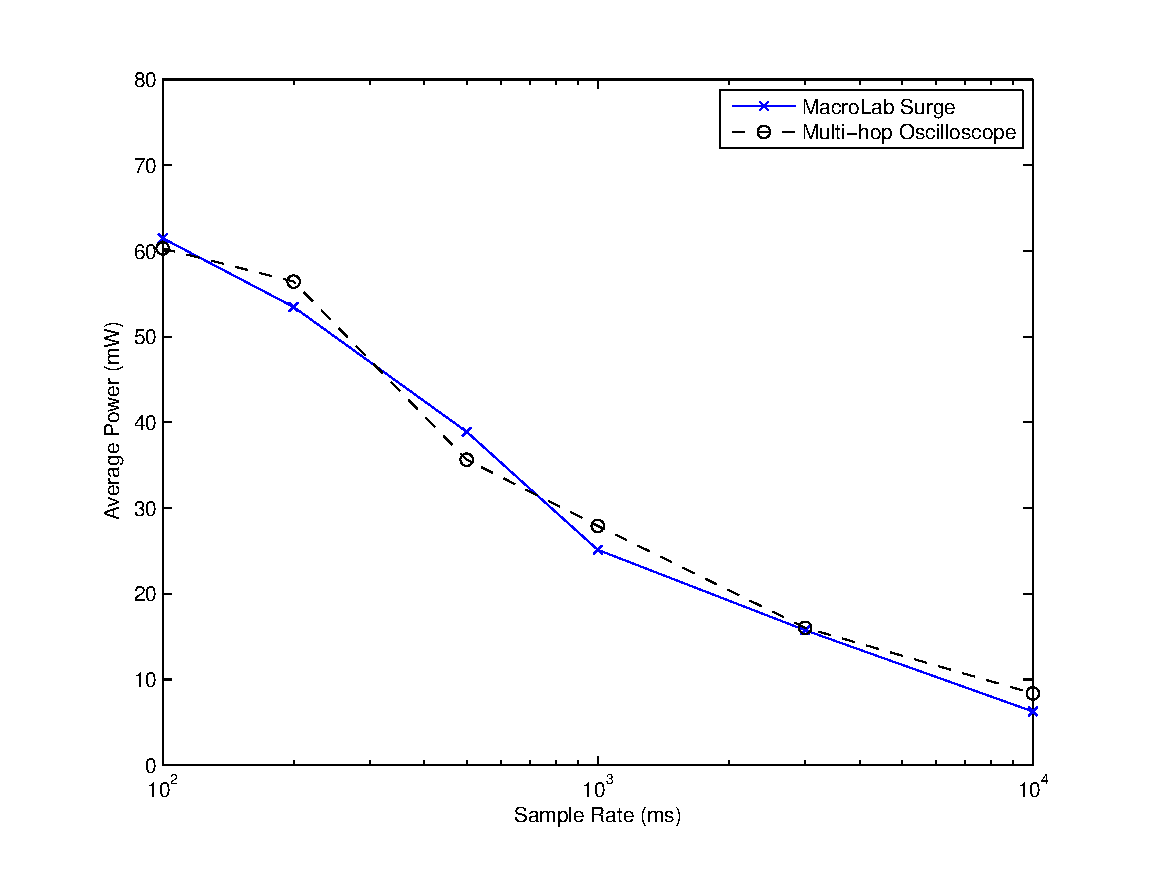
\includegraphics[width=1\columnwidth]{fig/SurgePower}
  \smallskip
  \hrule
  \caption{Oscilloscope power measurements of MacroLab and nesC Surge
  implementations.} 
  \label{fig:powerConsumption}
\end{figure}



\begin{table}
  \centering
  \begin{minipage}{\columnwidth}
    \centering
    \begin{tabular}{|l|r|r|r|}
      \hline
      \multicolumn{1}{|c}{Application}& 
      \multicolumn{1}{|c|}{Execution} &
      \multicolumn{1}{|c|}{CPU} &
      \multicolumn{1}{c|}{Stack}\\
      \hline
      Surge&17.7msec&361usec&120bytes\\
      \bf{MacroLab\_Surge}&18.2msec&705usec&124bytes\\
      \hline
    \end{tabular}
  \end{minipage}
  \smallskip
  \caption[Execution time analysis]{An evaluation of the execution time of the application, logic (CPU), and maximum
    consumed stack memory.}
  \label{table:ExecutionTime}
\end{table}


\subsection{Effect of DSCD on Performance}\label{sect:PerformanceEval}

\begin{figure*}[t]
  \begin{macrolab}
    RTS = RunTimeSystem();
    busstops = RTS.getNodes('stopnode'); 
    buses = RTS.getNodes('bus');
    estimates = Macrovector(busstops, length(buses) ,'uint16');
    arrivals = Macrovector(busstops, length(buses) ,'uint16'));
    travelTime = Macrovector(busstops, length(busstops), length(buses) ,'uint16'));
    busSensors = SensorVector('BusSensor',busstops,'uint16');
    routes = uint8({[1 2 3 4], [ 5 6 7 8]}); %Example routes

    while(1)
      [busID,r] =  sense(busSensors);
      busTime = RTS.getTime();
      travelTime(routes{r},routes{r},busID)[1,3] = busTime - arrivals(routes{r}, busID);
      arrivals(routes{r},busID)[1,2] = busTime;
      estimates(routes{r},busID) = travelTime(routes{r},routes{r},busID)[2,3] + busTime;
      BASE_DISPLAY(estimates(routes{r},:));
    end
  \end{macrolab}
  \smallskip
  \hrule width 2\columnwidth
  \caption{MacroLab code for the bus tracking application.}
  \label{code:BusTracking}
\end{figure*}

To evaluate the effect of DSCD on the performance of an application in multiple
scenarios, we implement a {\em bus tracking} application
(Figure~\ref{code:BusTracking}).  In order to easily modify the deployment
scenario, we performed this part of the evaluation in simulation.  In the bus
tracking application, each bus stop records arrival times for the buses and
computes estimated arrival times for all other buses. The application logic is
shown in Figure~\ref{code:BusTracking}, which maintains state about the last
time a bus was seen at every stop, the time it takes to travel from each stop to
every other stop, and the estimated time that each bus will next arrive at every
stop.

First, we sense for a bus at each stop and collect a time stamp of the bus
arrival as {\tt busTime}. The {\em arrivals} matrix stores the last time before
now that each bus arrived at each stop, so we update \textit{travelTime} to be
\textit{busTime} minus \textit{arrivals}. In other words, we estimate the travel
time between stops to be the current time that each bus arrived less the last
time that bus was seen at every other stop. \textit{Arrivals} is then updated
with the current arrival time of the bus. Next, the \textit{estimates} vector is
updated to be \textit{travelTime} plus \textit{busTime}. We estimate the
predicted arrival time for each bus to be its travel time plus the last time it
was seen at all stops. Finally, the estimated arrival times are displayed to
potential passengers using the {\tt BASE\_DISPLAY} operation.  These main matrix
operations in this application make heavy use of the dot product notation
described in Section~\ref{sect:dotProduct} for conciseness and efficiency.

MacroLab's row-level parallelism allows the matrix operations to occur
in parallel.  In this particular application, the program runs
correctly without using the synchronized implementation of any
inter-row operations, and so the assignment in line 15 does not block
until all values are collected.  Each row can be processed in parallel
as buses arrive at different stops.

\begin{figure}
  \centering
  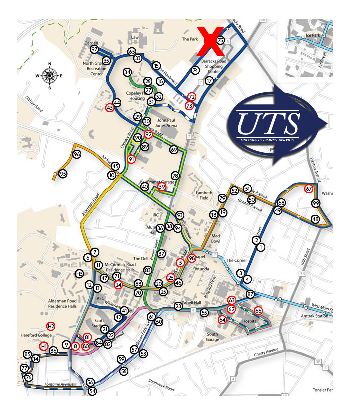
\includegraphics[width=.65\columnwidth]{fig/UTSBusRoutes}
  \smallskip
  \hrule
  \caption[UTS Bus Routes at U.Va.]{UTS Bus Routes at U.Va. The base station is indicated as a cross at
    the top of the figure.}
  \label{fig:UTS}
\end{figure}

We evaluate this application in four scenarios: 1) the estimated bus arrival
times are displayed to the passengers on a website which is updated from a
centralized base station, 2) the estimated bus arrival times are displayed to
the passengers at each bus stop, 3) the base station radio range is increased
substantially for better coverage, and 4) an additional bus route is added by
the bus company.  Our results show no decomposition is best for all target
deployments and choosing the correct decomposition can reduce messaging
costs by an average of 44 percent.

MacroLab can optimize for a number of cost metrics (such as latency,
power consumption, or message cost) by using a cost profile and a
cost analyzer that analyzes the cost of each program decomposition for a
target deployment scenario. In this evaluation, we only optimize the
total number of messages that must be sent by the network to achieve the
global objective. 

\subsubsection{Experimental Setup}\label{sect:setup}
Our test scenario consists of actual bus routes at the University of Virginia,
provided by the University Transit Service (UTS), shown in Figure~\ref{fig:UTS}.
We assume that each bus stop has a mote and can sense the bus currently at its
stop.  The cost profile of the test scenario was created based on the actual
locations of the bus stops and assuming a reliable communication range of 500 meters

In order to test this wide variety of deployment scenarios, we built a
Matlab-based simulator for this part of the evaluation.  The
simulation environment for MacroLab only requires a slight
modification to the RTS in order to support function calls into the
simulator instead of directly to the nodes.  The simulator runs code 
similar to microcode that would run on a mote-based RTS.  In this
experiment, we only evaluate two decompositions: a centralized and
distributed decomposition.

Communication between nodes is provided by the RTS. Based on the cost profile
of the network, the simulation observes the total message cost for each
decomposition and scenario.  The cost matrix is computed from the topology
of our scenario and encodes the cost to send messages between pairs of nodes.
The RTS currently supports point-to-point routing but more routing algorithms
can be added as they are developed.

\begin{figure}[t]
  \centering
  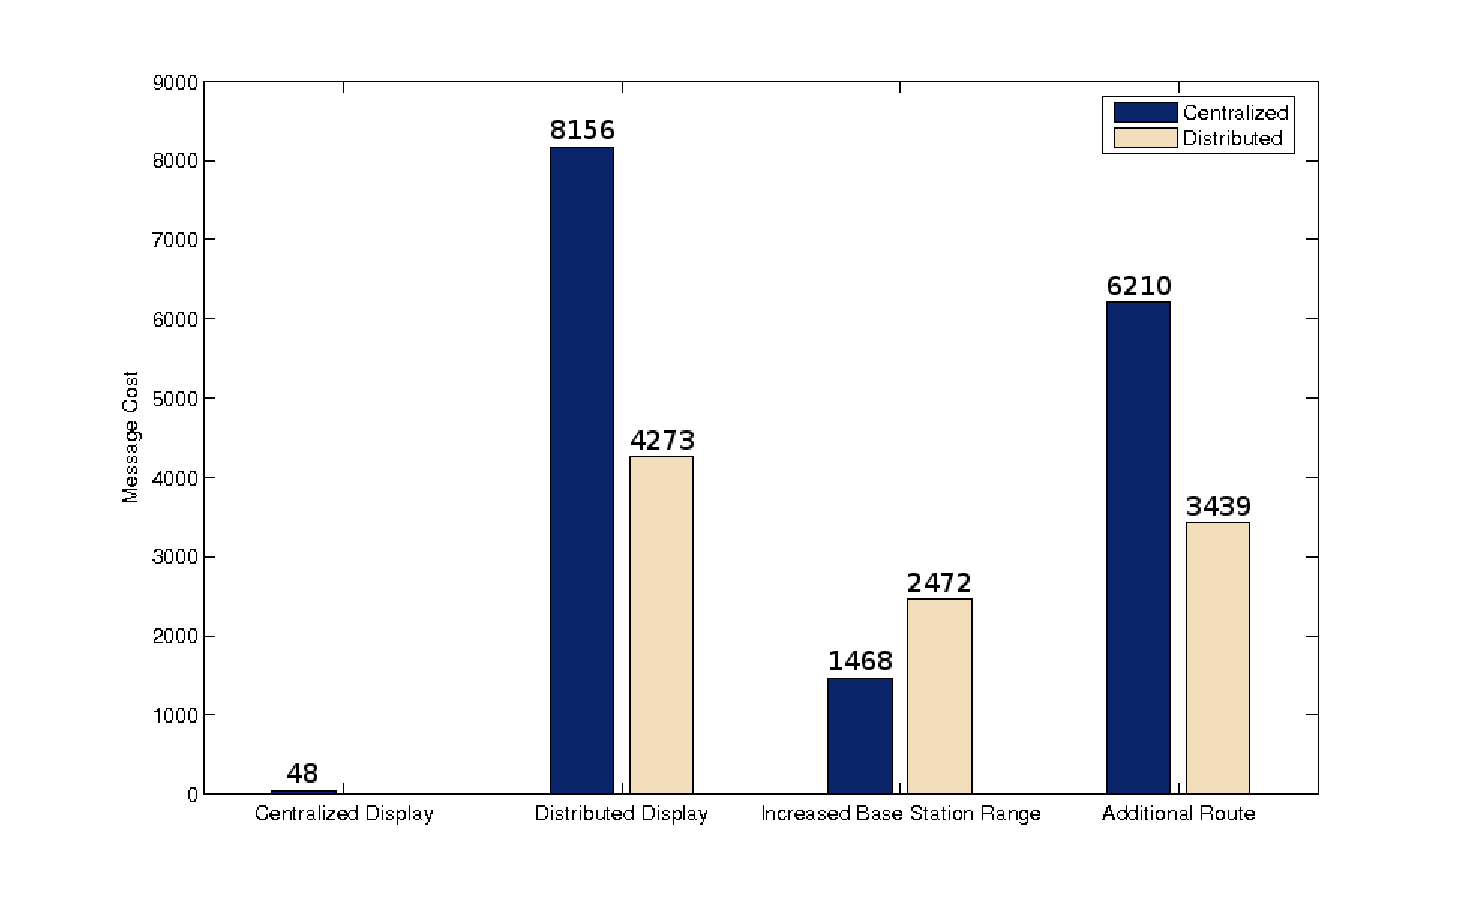
\includegraphics[width=1\columnwidth]{fig/scenarioSmall}
  \smallskip
  \hrule
  \caption[Effect of deployment scenario on efficient implementation]{Neither
    decomposition is best for all deployment scenarios. Small changes in the
    deployment scenario changes the optimal implementation between centralized
    and distributed.}
  \label{fig:MainResult}
\end{figure}

\subsubsection{Scenario 1: Website Display} 

In the first scenario, we record and display the bus information on a website
using a centralized base station.  This is accomplished by using the {\tt
  BASE\_DISPLAY} operation which can only be executed in a centralized fashion.
In order to accomplish this version of the application, the nodes will sense
buses and send their data directly back to the base station which will maintain
state in all of the macrovectors and perform all of the vector computations.
The messaging cost of this application is the same as the Surge
application.  Only one bar is shown in Figure~\ref{fig:MainResult} because the
{\tt BASE\_DISPLAY} operator is only defined for centralized decompositions.  By
running this decomposition in simulation, we found the cost of running the
application using this scenario to be 48 messages over a 30 minute simulation.

\subsubsection{Scenario 2: Bus Stop Displays} 

Changing {\tt BASE\_DISPLAY} to {\tt MOTE\_DISPLAY} allows us
to show the data at each bus stop rather than at the base station. Sending
and receiving bus arrival information between all nodes within each route totals
8156 messages for the centralized implementation and 4734 for the distributed
version; the distributed decomposition is almost twice as efficient.  The large
increase in the number of messages is due to the fact that each time a bus arrives at a stop,
its arrival time must be transmitted to all the stops in the route. In the
centralized implementation, this requires $O(n^2)$ messages per route, where $n$
is the number of stops on that route. This cost increases dramatically for
routes that are far from the base station. All nodes must send each bus arrival
event all the way to the base station which must then forward the message back
to each node on the route individually.

\begin{figure}
  \centering
  \includegraphics[width=0.8\columnwidth]{fig/Decomposition}
  \smallskip
  \hrule
  \caption{Macrovectors in centralized and distributed implementations.}
  \label{fig:Decomposition}
\end{figure}

The cost of the distributed implementation does not incur this overhead. Each
node forwards bus arrival events to all other nodes on its route; it does not
need to transmit back and forth to the base station.  If a stop is
on two or more routes, it forwards the message to all other stops on all such
routes.  In the compiled code, this is achieved by distributing all vectors in
the program and making the {\tt arrivals} vector a reflected vector across all
nodes on a route. The difference in macrovector storage between the centralized
and the distributed decompositions is shown in Figure~\ref{fig:Decomposition}.
For this target deployment scenario, the messaging cost of the distributed
decomposition is about 50 percent lower than the centralized decomposition.

The only change to the bus tracking application in this scenario versus
Scenario~1 is that the {\tt BASE\_DISPLAY} function was changed to {\tt MOTE\_DISPAY},
changing the library function from a centralized operator to a distributed
operator.  It should be noted that if this were a TinyOS application, we would
be required to implement a completely new version of the program in order to
make this change.  Thus, small changes in the program can result in large
changes to the cost profile of each decomposition.  In MacroLab, the single line
addition is handled by the decomposer and the RTS in order to choose the optimal
solution.

\subsubsection{Scenario 3: Increased Base Station Range}

\begin{figure}
  \centering
  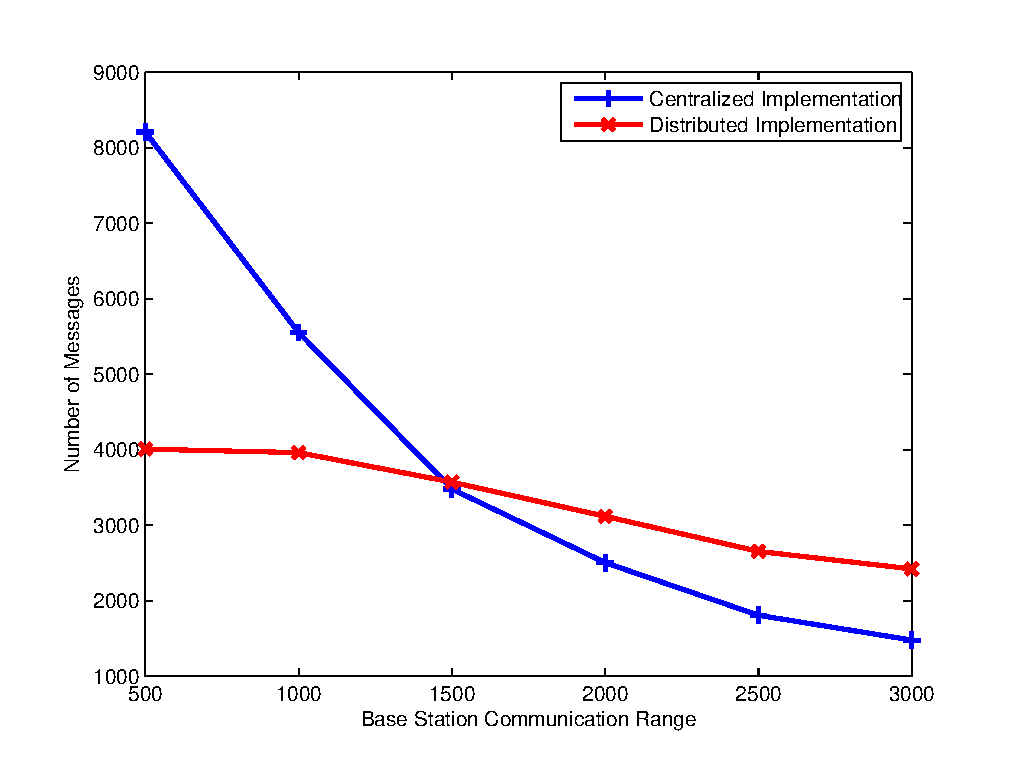
\includegraphics[width=1\columnwidth]{fig/RangeCompare}
  \smallskip
  \hrule
  \caption{Changing the base station range changes the balance
  between the two decompositions.}
  \label{fig:RangeCompare}
\end{figure}

In the third deployment scenario, a high-gain antenna is added to the
base-station which increases the coverage of the base station and changes
the cost profile of the network.  Figure~\ref{fig:MainResult} shows that
adding the antenna reduces the cost of messages dramatically.  This cost
reduction is because the increased range allows all of the nodes to more
cheaply communicate with the base station.  However, this change affects
the centralized decomposition to a greater extent.  This is because all nodes in the
network use the base station link in the centralized implementation while
in the distributed implementation, only the nodes that can
opportunistically route through the base station to reduce messaging costs
to other nodes on the route will actually do so.  Increasing the base
station range increases the number of nodes that opportunistically route
through the base station, reducing messaging costs but not as dramatically
as in a centralized decomposition. Figure~\ref{fig:RangeCompare} shows
that for more then a 1500 meter range, the centralized implementation gives superior
performance. 

In this scenario, a centralized decomposition costs 1468 messages while the
distributed version costs 2472 messages. This is a reversal of the cost
trade-off in the previous scenario. We show that small changes to radio
hardware can lead to large changes in the cost profile of the target
deployment. Redesigning a TinyOS program to be efficient given this new
cost profile would be difficult, but the MacroLab framework makes this
change automatically.

\subsubsection{Scenario 4: Additional Route} 
\begin{figure}
  \centering
  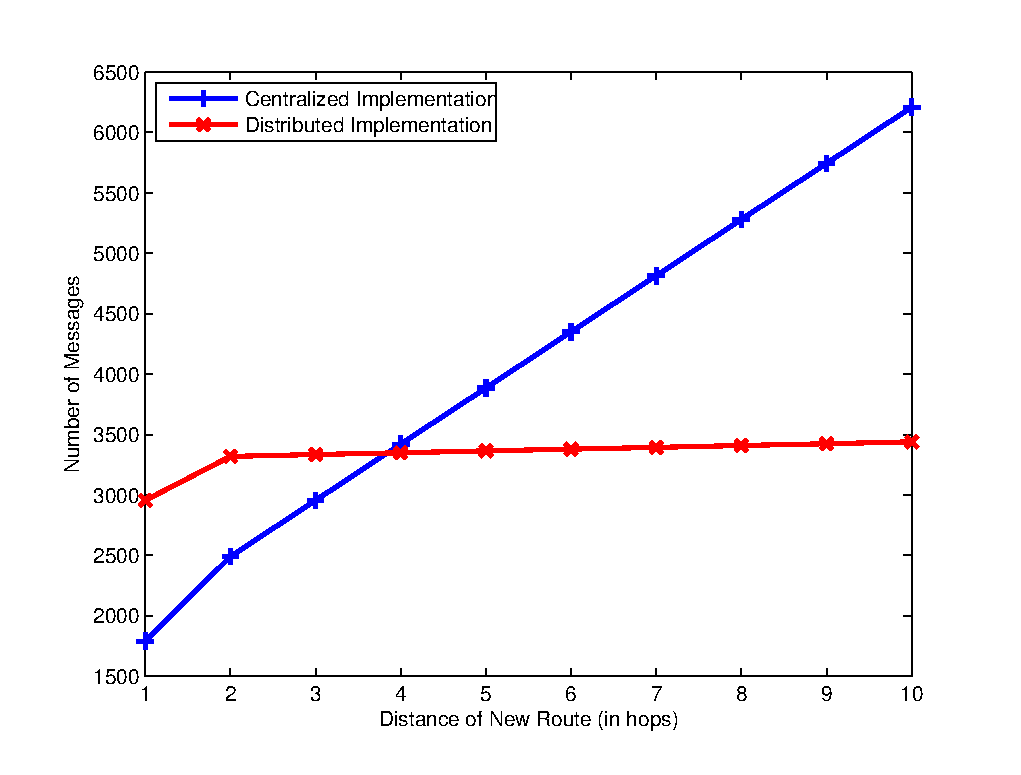
\includegraphics[width=1\columnwidth]{fig/MovingRoute}
  \smallskip
  \hrule
  \caption[Effect of adding a route to bus tracking application]{Adding a new
    route at various distances changes the balance between the two
    decompositions.}
  \label{fig:MovingRoute}
\end{figure}

In the fourth deployment scenario we add a route that runs from the main
campus to a new location 2500 meters away from the base station.
Figure~\ref{fig:MovingRoute} shows the distributed and centralized costs
as a function of the number of hops from the base station. As the number of hops
increases, the centralized decomposition must send messages farther to
reach the base station, while the cost of the distributed decomposition
does not change. Once this messaging cost to and from the base station
exceeds the cost of sending messages directly to the other nodes in the
route, it is more expensive to utilize the centralized implementation.

Figure~\ref{fig:MainResult} shows that at an additional 4000 meters, the
distributed version becomes more efficient than the centralized
decomposition. The centralized cost is 6210 and the distributed cost is
3439.  Because the new route is farther away from the base station,
communication with the base station becomes more expensive.  In this
scenario, we demonstrate that small changes to the network topology can
cause large changes to the cost profile of the target deployment.

\subsection{Accuracy of Static Cost Analyzer}
\label{sect:analysisAccuracy}
\begin{figure}
  \centering
  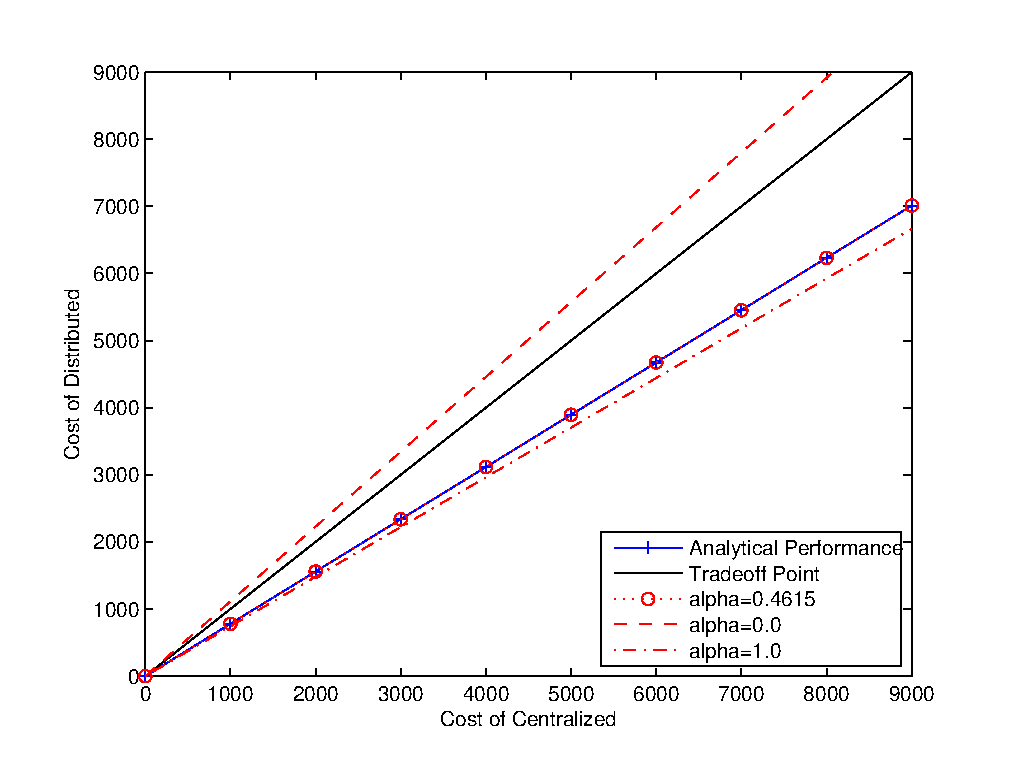
\includegraphics[width=1\columnwidth]{fig/Buses}
  \smallskip
  \hrule
  \caption[Estimated and measured messaging costs.]{The parameter
  $\alpha$ is the ratio of buses on long routes versus those on all
  other routes. The actual distribution of bus detection events can change the
  true messaging cost within a narrow range around the statically estimated cost.
  }
  \label{fig:Buses}
\end{figure}

Our static cost analysis (Section~\ref{sect:staticCost}) can make
use of information about expected event frequency. For simple event-loop
MacroLab programs, the presence and quality of this event frequency
information is the determining factor in the accuracy of the analysis.
In the worst case, such information is not available. For the bus
tracking application, lacking any other information, our static analysis
assumes that each bus stop observes a bus event with the same frequency.
However, this is not necessarily true and there will be some
discrepancy between the cost estimated by the static analysis and the
actual cost of the decompositions. For example, if a larger percentage
of buses appear on very long routes, this will increase the cost of the
distributed decomposition relative to the static estimate. On the other
hand, if many buses appear on routes far from the base
station, this would increase the cost of the centralized decomposition.

Figure~\ref{fig:Buses} shows static estimated costs as well as dynamic
measured costs as the distribution of buses and therefore sensed events
within the network changes.  To highlight the differences between the
centralized and distributed implementations, we focus on the longest
routes. The parameter $\alpha$ is defined as the ratio of buses on the
long routes versus those on all other routes.  The crossover
point for centralized and distributed message costs is represented by
the $y=x$ line.  Ratios above the crossover line will be optimally run
as centralized applications, those below as distributed.  By
computing the ratios for various scenarios, we can see how much each
change will affect the total cost of the application and whether it will
cause a switch in the optimal implementation.  The bounds of our application
are plotted by the $\alpha = 0$ and $\alpha = 1$ lines, in which either
all buses or no buses appear on the longest routes. Our static cost
analysis algorithm is quite accurate for this application and is not
extremely sensitive to the assumptions made about the frequency of
events; it will only be incorrect with extremely non-uniform event
distributions.  In such cases, the run-time system can dynamically
monitor changes or errors in the cost profile of the target deployment.
As shown in Figure~\ref{fig:System}, such dynamic cost information can
be fed back into the cost analyzer which can decide to reprogram the
network.


\section{MDB} \label{mdbEvaluation}

We evaluate MDB in two parts. First, we show that data traces
are more effecient for macrodebugging than the traditional approach of creating
event traces.  Then, we evaluate the RAM, flash, energy, and CPU cycle overhead
of MDB\@.

\begin{figure}[t]
  \centering
  \includegraphics[scale=1]{fig/testbed}
  \caption[Evaluation testbed with 21 Tmote Sky motes]{We evaluated MDB on three
  macroprograms by running them on a 21 node testbed. Light sensors and a
  projector created the sensor stimuli.}
  \label{fig:testbed}
\end{figure}

\subsection{Experimental Setup}
The evaluations were carried out on a testbed with 21 TMote Sky nodes with
photoresistor sensors (Figure~\ref{fig:testbed}). Since all the nodes in the
testbed are within one hop of each other, we artificially limit their
communication ranges by modifying the packet reception module of the CC2420
radio. We restrict nodes to communicate with neighbors next to them vertically,
horizontally, and on the two diagonals.  To collect additional data that could
not be obtained from the testbed, we used the node-level Cooja network
simulator~\cite{Osterlind2006} which makes use of the MSPSim~\cite{Eriksson2007}
TMote Sky simulator.  The microcode executing on the nodes in the Cooja
simulator is exactly the same microcode that executes on the real \tmotesky
hardware.

We evaluated MDB with three macroprograms.  The first application is OTA,
described earlier (Figure~\ref{code:ota}), for which we emulated the movement of
objects using the light sensors by moving a white circle on a black background
that was projected from a laptop onto the testbed. The intensity of the circle
decreases radially outward to emulate the effect of varying sensor readings by
nodes that detect the object.  The second application is Surge
(Figure~\ref{code:surge}), which is a simple data collection application that
periodically samples from a sensor and displays the readings at a base station.
The third is an acoustic monitoring application (Figure~\ref{code:acoustic}),
which first senses from a microphone sensor, and depending on the number of
neighbors that also heard a sufficiently loud sound, samples from a second
high-fidelity microphone, stores the values, and reports them to
the base station.  The sensor values for both of these applications are
generated using the photoresistors on the nodes.

\begin{figure}[t]
\begin{macrolab}
every(uint16(1000))
 lightVals = lightSensor.sense();
 basedisplay(lightVals);
end
\end{macrolab}
\caption[The macroprogram for Surge]{Surge reads sensor values and displays them
at the base station.}
\label{code:surge}
\end{figure}

\begin{figure}[t]
\begin{macrolab}
every(uint16(1000))
 trigger = microphone.sense();
 meanTrigger = mean(neighborTrigger, 2);
 candidates = find(meanTrigger > THRESHOLD);
 soundLog(candidates) = microphoneHF(candidates).sense();
 baselog(soundLog);
end
\end{macrolab}
\caption[The macroprogram for acoustic monitoring]{The acoustic monitoring
application reads values from a microphone and reads from a higher-fidelity
microphone on nodes whose neighborhoods detect high average noise levels.}
\label{code:acoustic}
\end{figure}

\subsection{Data vs. Event Logging} \label{dataEvent}

\begin{figure}[t]
  \centering
  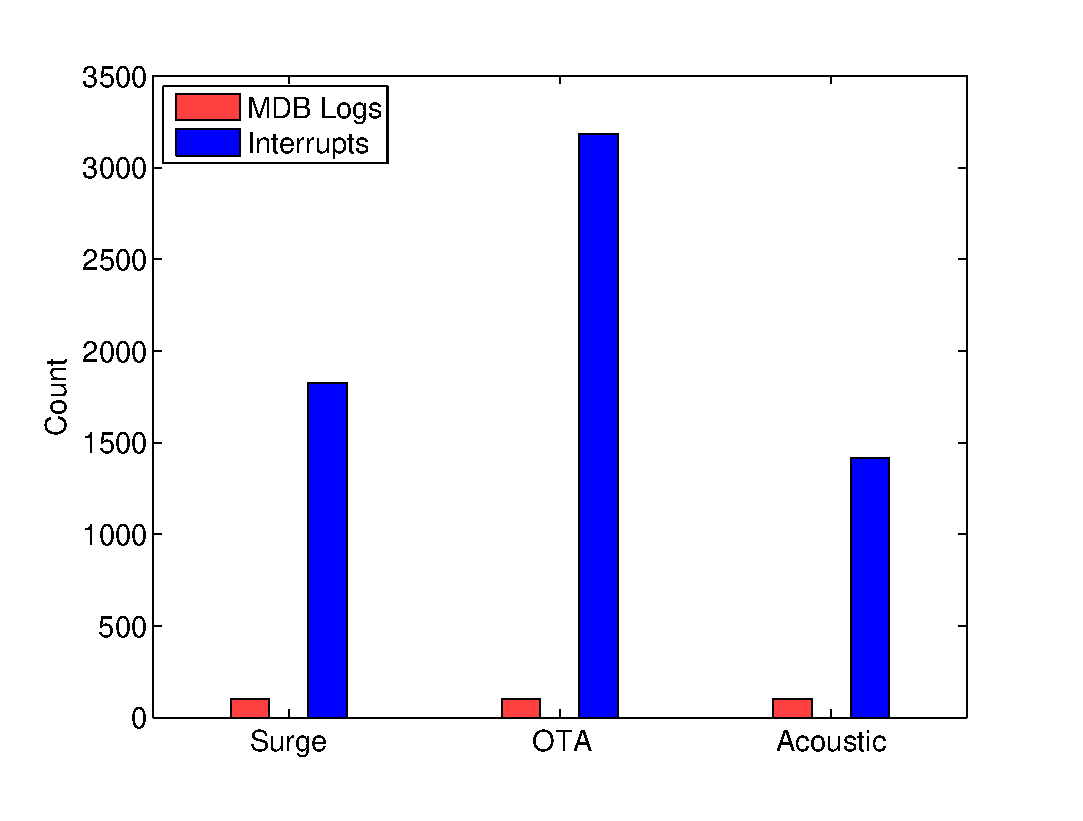
\includegraphics[scale=0.75]{fig/interruptvsMLLogger}
  \caption[Number of interrupts generated per 100 data states written to
  flash]{Number of interrupts generated per 100 data states written to
  flash. WEN applications produce 14--32 times more interrupts and message
  events than macroprogram state updates.}
  \label{fig:interruptvsMLLogger}
\end{figure}

We evaluate the cost of creating data traces by counting the number of logging statements
required to record all variable writes and program counter changes for a single
run of each of the three macroprograms. We compare this count to the number of
interrupts that would need to be logged to create an event trace of the same
program execution.  Since we could not count the interrupts generated on real
hardware without changing the timing characteristics of the program, we obtained
these values by analyzing the programs as they executed on the Cooja network
simulator.  Figure~\ref{fig:interruptvsMLLogger} shows that, for these
applications, the number of hardware interrupts is 14--32 times larger than the
number of updates to macroprogram state.  These results clearly show that MDB's
approach of collecting data traces is much more efficient for macroprograms than
the traditional approach of collecting event traces.

\subsection{RAM and Flash Overhead} \label{overhead}

\begin{figure}[t]
  \centering
  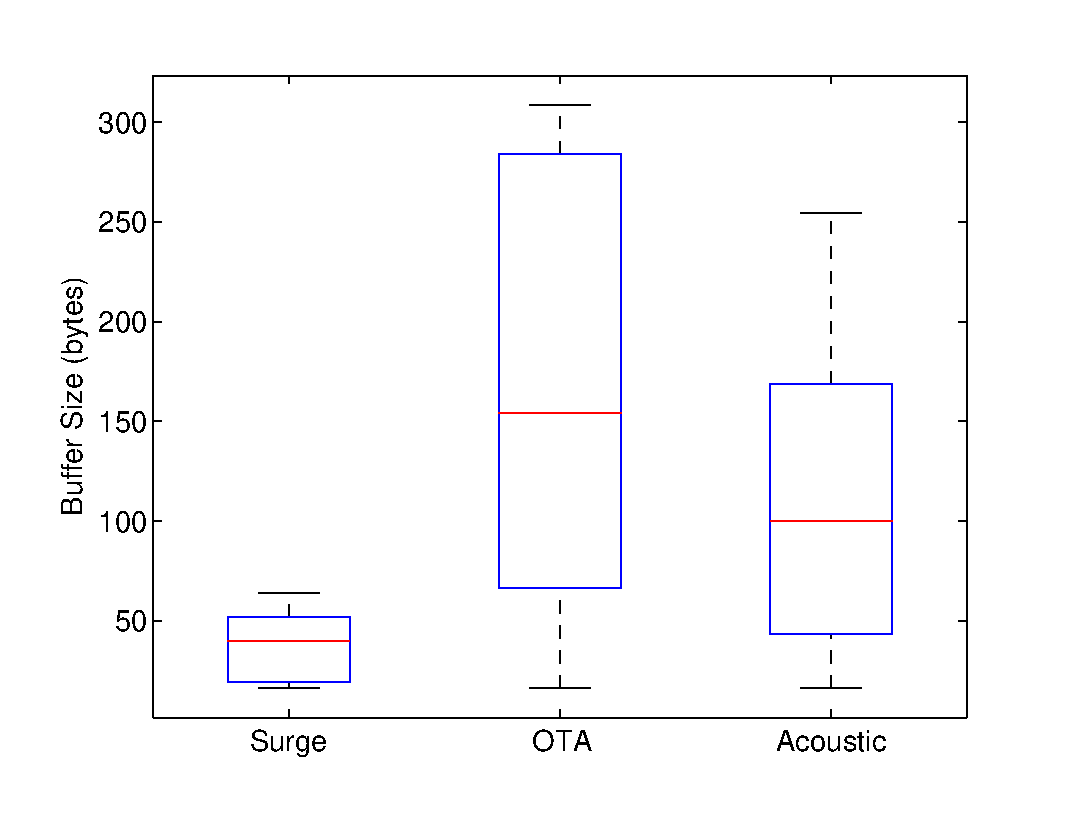
\includegraphics[scale=0.75]{fig/bufferSize}
  \caption[RAM Overhead]{Log data is stored temporarily in RAM before being written to flash.
    In our experiments, no node needed more than 304 $Bytes$ of RAM\@. The box plot
    shows the minimum, lower quartile, mean, upper quartile, and maximum
    values.}
  \label{fig:bufferSize}
\end{figure}

\begin{table}
  \centering
  {
    \begin{tabular}{|l|r|r|} \hline
      Application & Flash ($Bps$) & Wraparound ($hr$)\\ \hline\hline
      Surge & 31 & 9 \\ \hline
      Accoustic & 187 & 2 \\ \hline
      OTA & 288 & 1 \\ \hline
  \end{tabular}}
  \caption[Flash memory consumption]{Flash memory consumption is low enough to debug hours of
      execution. The buffer is circular, so it can always store data to debug the
      last few hours of execution.}
  \label{table:flashCapacity}
\end{table}

Memory is not typically a concern for traditional debuggers that execute on PCs,
but WENs are composed of highly resource-constrained devices and efficient
memory usage is essential to making MDB practical in this domain.  We measured
the amount of memory MDB requires by instrumenting the RAM buffer portion of
the logger and tracking the maximum difference between the head and tail
pointers of the circular buffer. Figure~\ref{fig:bufferSize} depicts box plots
that show the minimum, maximum, mean, and the lower and upper quartiles of RAM
consumption for each of the three test applications executing on our 21 node
testbed. This data reveals that MDB has modest RAM requirements, and needs to
store a maximum of 304 $Bytes$ of data, while the \tmotesky nodes have about 10\KB
of RAM available.

We also measured the amount of Flash memory required by MDB to store the
complete data traces for each of the three applications.
Table~\ref{table:flashCapacity} shows that the applications store less than
300 $Bps$ to the flash.  At these rates, simple applications such as Surge can
collect logs for several hours before exhausting the $1 \ MB$ of external flash
available on the \tmotesky.  More complicated applications such as OTA and
acoustic monitoring may exhaust the flash after about one and a half
hours. Thus, bugs in these applications must be detected within one and a half
hours in order to debug them before the log entries are overwritten.

\subsection{CPU Overhead} \label{CPUoverhead}

We evaluate the effect of MDB on execution speed by counting the logging
instructions executed during a particular run of the three applications. Since
it was difficult to collect this information from the actual nodes without
substantially modifying the timing characteristics of the application, this data
was collected by running the application on the Cooja simulator. Since Surge has
no interaction between nodes, we simulated it using 1 node.  Acoustic monitoring
used 5 nodes and OTA used 10 nodes.  Figure~\ref{fig:execBreakdown} shows the
number of MacroLab application instructions and MDB logging instructions that
execute, as a percentage of the total execution time. The values in
Figure~\ref{fig:execBreakdown} are averages over all the nodes simulated in
Cooja. As Figure~\ref{fig:execBreakdown} shows, the MacroLab application code
executes for between 2\% and 6\% of the total execution time and the logging
code executes for less than 0.5\% of the total execution time.

\begin{figure}[t]
  \centering \includegraphics[scale=0.75]{fig/execBreakdown}
  \caption[CPU Overhead]{MacroLab context constitutes less than 6\% of all code running on
      the nodes. Logging code constitutes less than 0.5\%.}
  \label{fig:execBreakdown}
\end{figure}

It takes exactly 105 machine instructions to log data to the RAM buffer.
Execution is minimal because on the MSP430 an instruction takes approximately
125 nanoseconds.  This means the logging overhead is about 13 microseconds.
This is extremely small when compared to the normal duty cycle of applications
written in MacroLab.

\subsection{Energy Consumption} \label{PowerConsumption}

We evaluate MDB's energy consumption by executing the OTA application, with the
senor being sampled every $10$ seconds, on the 21 node testbed and measuring its
average current draw over a period of $100$ seconds.  We executed this
experiment with MDB, MDB-lite, and without MDB\@.  We repeated the experiment
both with and without low-power listening
(LPL)~\cite{Polastrea}. Figure~\ref{fig:powerConsumption} shows that an
application consumes 30\% more energy with MDB, when LPL is enabled with a sleep
interval of $1$ second.  This energy overhead is due to the process of saving
logs to the external flash chip. With MDB Lite, this overhead is reduced to only
0.2\mW or 0.9\%.  This is because MDB Lite does not write to flash, and the
timer-based implementation of MDB Lite allows the node to sleep when possible.
The overhead of MDB and MDB Lite when LPL is disabled is only 0.5\mW because the
node does not go into sleep mode in any of these implementations.

\begin{figure}[t]
  \centering \includegraphics[scale=0.75]{fig/energy}
  \caption[Energy Consumption]{Without low-power listening enabled, applications
  consume 30\% more energy with MDB enabled, but only 0.9\% more energy with MDB
  Lite. }
    \label{fig:powerConsumption}
\end{figure}

\subsection{Discussion} \label{discussion} 
%
The effectiveness of MDB as a CPS debugger depends on two factors: (i) the
usefulness of the debugging abstraction and (ii) the efficiency of trace
logging. We attempt to address the first factor by demonstrating that the
features of MDB can be used to debug three classes of bugs in macroprograms
(Chapter~\ref{Interface}). MDB, by its very nature, does not enable the
debugging of bugs in layers below the application layer. For example, a user
cannot identify a bug in the MAC layer or routing layer because MDB hides
message passing between nodes. This abstraction of low-level details conforms to
the abstraction provided by the macroprogramming system since one of the goals
of MDB is to allow the user to program and debug at the same level of
abstraction. Also, MDB relies on the guarantees of macroprogramming systems that
the low-level libraries have been rigorously tested and can be used in
macroprograms to build more complicated applications. If a user of a
macroprogramming system does not have such a guarantee about the function
libraries, macroprogramming would become more of a burden on the user than
writing the functions from scratch as the user would have to test the
interoperability of various functions, that have been written by others, before
they can be used to write an application. Thus, a debugger that allows the user
to debug at the application level of a macroprogramming language is a useful
debugging abstraction.

In order for MDB to be useful, execution traces should be collectible for a
sufficient duration. MDB attempts to maximize the duration of execution for
which traces can be collected by minimizing the number of trace entries that
have to be logged per unit of time. This is done by exploiting the fact that the
user is debugging at the macroprogram abstraction and, therefore, only changes
that are reflected in the macroprogram need to be logged. Thus, the many events,
such as interrupts, that take place in the TinyOS operating system for instance
can be ignored since they are not visible at the macroprogramming
abstraction. What MDB does log are the writes to variables declared in the
macroprogram a macroprogram counter than indicates which part of the
macroprogram each node is executing. This enables MDB to log 14--32 times fewer
trace entries per unit of time than if MDB were logging all events within a node
so as to recreate each node's execution. 

MDB utilizes a temporary buffer in RAM to which macroprogram state changes are
logged while each iteration of the macroprogram's every loop is executing. At
the end of each iteration, this buffer is written to flash. The amount of RAM
required for MDB depends on the number of variables in the macroprogram, the
number of lines of code in the macroprogram, and the number of neighbors with
which each node shares macrovectors. Our evaluations indicate that for OTA,
which has 13 lines of macrocode with five vectors, on the 21 node testbed where
each node has eight neighbors the maximum amount of RAM required is 304
$Bytes$. This is just $3\%$ of the RAM available on Tmote Sky nodes. While
larger, more complicated applications could require a greater amount of RAM for
the buffer, the fact that OTA, which is one of the largest and most complicated
WEN applications to data~\cite{Whitehousea}, requires such a small fraction of
the available RAM indicates that MDB would not pose much of an overhead on the
available RAM for most applications.

For the duration of the data collection phase the traces are stored on the
node's external flash. For the object tracking application traces for one hour
of execution can be collected before the flash buffer gets overwritten. This
duration can be increased for debugging purposes by reducing the sampling
frequency or network density which would decrease the number of state changes
that have to be logged. For most applications which would fall in the complexity
spectrum between Surge, which is one of the simplest WEN applications, and OTA,
around five hours of execution traces could be collected without overwriting the
flash. For most WEN applications, five hours of execution should be sufficient
during the debugging phase to analyze their performance and identify bugs. If
the user needs data from a longer execution of the application, the traces can
be collected periodically, just before the flash buffer gets overwritten, and
the application could be allowed to continue executing.

Due to the controlled conditions under which the testing phase of application
development usually takes place, the limitations placed by the flash capacity
can be overcome as described above. Yet, if the user wishes to deploy the
application with logging enabled so that any bugs that arise during deployment
can be analyzed, the flash capacity is of greater concern. For example, the
presence of a bug in a data collection application may only be noticed when the
data is analyzed at the end of a deployment. MDB may not be usable for
identifying this bug if the bug occurred before the last $n$ hours of execution
if the flash buffer fills up every $n$ hours. Yet, if the bug manifested itself
within the last $n$ hours, the available data traces could still be used with
MDB to identify the bug. This would not be possible if MDB logged execution
traces without resorting to checkpointing or other techniques for storing the
state of the system periodically.

MDB impacts the execution speed of applications by consuming CPU cycles to carry
out the logging operation. As Figure~\ref{fig:execBreakdown} shows logging to
RAM imposes only a $0.5\%$, or 13\us, overhead on the application execution
time. Since the inherent uncertainty of even a sensor readings is an order of
magnitude greater at 20 ms (Section~\ref{time}), the 13\us overhead of logging
can be ignored for almost all applications.

MDB also consumes energy while logging which could decrease the lifetime of the
application. As Section~\ref{PowerConsumption} describes, an application with
logging enabled consumes 30\% more energy than the application without logging
enabled. This is a considerable amount of energy since it could decrease the
lifetime of a system by 30\%, for instance causing an application that could
have executed for a year to die in eight months. A user could mitigate this
issue in two ways. The first is to increase the power available to each node by
at least 30\%. This can be done by providing each node larger or additional
batteries or augmenting each node with energy scavenging capabilities. This
would enable the full logging capabilities of MDB to exist while the application
is executing in the real world so that if a problem were to arise the user could
obtain the traces and attempt to identify its cause. 

An alternative is to deploy applications in two phases. The first is a debugging
phase where the application, with MDB logging enabled, is deployed for a short
period of time so that traces can be collected and bugs identified. Then, after
the identified bugs have been fixed, the application is deployed for its full
duration without the MDB logging capabilities enabled so that their is no energy
overhead. This is ideal if the application does not need logging during
execution or if it providing each node with additional power is not feasible and
the application cannot tolerate the energy overhead of MDB. Yet, an application
without MDB logging enabled could behave differently from an application with
MDB logging enabled due to the difference in timing between the two. This is
mainly the time MDB take to write the RAM buffer to flash which could be about
10 ms per log entry. This timing difference could cause a bug that was hidden
when MDB was enabled to manifest itself during the actual deployment. Such bugs
are called Heisenbugs. MDB allows a user to deploy an application without flash
writing enabled while still maintaining the timing characteristics of MDB by
enabling MDB Lite instead of MDB when compiling the application. MDB Lite
functions just like MDB except when writing the RAM buffer to flash. During this
phase MDB Lite disables the interrupts which MDB disables when writing to flash
and puts the node into a sleep state for the same duration of time MDB takes to
write the RAM buffer to flash. This operation ensures that MDB Lite behaves in
an identical manner to MDB in terms of timing, yet by eliminating the flash
writes decreases the energy overhead from 30\% to 0.9\% which should be
tolerable for most applications. Thus, as other projects such
as~\cite{Ronsse2001} have claimed, MDB eliminates the possibility of Heisenbugs
by enabling the tracing to be left on at all times.




% LocalWords:  TinyOS Matlab RTS macroprogram MacroLab Agilla EnviroSuite RPC
% LocalWords:  AlarmNet basicstyle numberstyle breaklines breakautoindent numel
% LocalWords:  RunTimeSystem lightSensors createSensorVector LightSensor DSCD
% LocalWords:  lightValues BASEDISPLAY magVals Macrovector neighborMagVals UTS
% LocalWords:  neighborReflection MagnetometerSensor leaderID CAMERAFOCUS busID
% LocalWords:  macrovector busTime travelTime busstops getNodes stopnode DISPAY
% LocalWords:  busSensors BusSensor getTime macrovectors nesC LOC
